\vspace{1.5cm}
\section*{Exercise 2: Slackness Theorem}
\begin{enumerate}
    \item Find the dual of the below primal :\\[0.15cm]
\[\text{min } Z = 3x_1 + x_2 + x_3\]
\vspace{-0.25cm}
\[
\left\{
\begin{array}{l}
    x_{1} + 2x_{2}  \geq 8 \\
    3x_{1} - x_{2} + x_{3} \geq 6 \\
    x_{1}, x_{2}, x_{3}\geq 0
\end{array}
\right.
\]

\vspace{0.15cm}
    \item Solve the dual
    \item Using the slackness theorem find solution of primal from solution of the dual
\end{enumerate}

\vspace{1cm}

\subsection*{\underline{Solution}}

\vspace{0.25cm}
\subsubsection*{\underline{Primal}}
\[\text{min } Z = 3x_1 + x_2 + x_3 \quad\Longrightarrow\quad  \text{max } -Z = -3x_1 - x_2 - x_3\]

\vspace{0.1cm}
\[
\left\{
\begin{array}{l}
    x_{1} + 2x_{2}  \geq 8 \\
    3x_{1} - 2x_{2} + x_{3} \geq 6 \\
    x_{1}, x_{2}, x_{3}\geq 0
\end{array}
\right.
\quad\Longrightarrow\quad
\left\{
\begin{array}{l}
    -x_{1} - 2x_{2}  \leq -8 \\
    -3x_{1} + 2x_{2} - x_{3} \leq -6 \\
    x_{1}, x_{2}, x_{3}\geq 0
\end{array}
\right.
\]

\newpage
\[
X = \left[\begin{matrix} x_1 & x_2 & x_3 \end{matrix}\right], \hspace{0.35cm}
C = \left[\begin{matrix} -3 & -1 & -1 \end{matrix}\right], \hspace{0.35cm}
b = \left[\begin{matrix} -8 \\ -6 \ \end{matrix}\right], \hspace{0.35cm}
Y = \left[\begin{matrix} y_1 & y_2  \end{matrix}\right]
\]

\vspace{0.5cm}

\[
A = \left[\begin{matrix}   -1 & -2 & 0 \\
                           -3 & 2 & -1
                           \end{matrix}\right], \hspace{0.35cm}
        A^{T} = \left[\begin{matrix}  -1 & -3   \\
                                      -2 & 2 \\
                                      0 & -1 
                     \end{matrix}\right]
\]

\vspace{0.5cm}
\subsubsection*{\underline{Dual}}
\[\text{min } Z = -8y_1 - 6y_2 \]

\[
\left\{
\begin{array}{l}
    -y_{1} - 3y_{2} \geq -3 \\
    -2y_{1} + 2y_{2}  \geq -1 \\
     -y_{2}  \geq -1 \\
    y_{1}, y_{2}\geq 0
\end{array}
\right.
\]

\begin{center}
    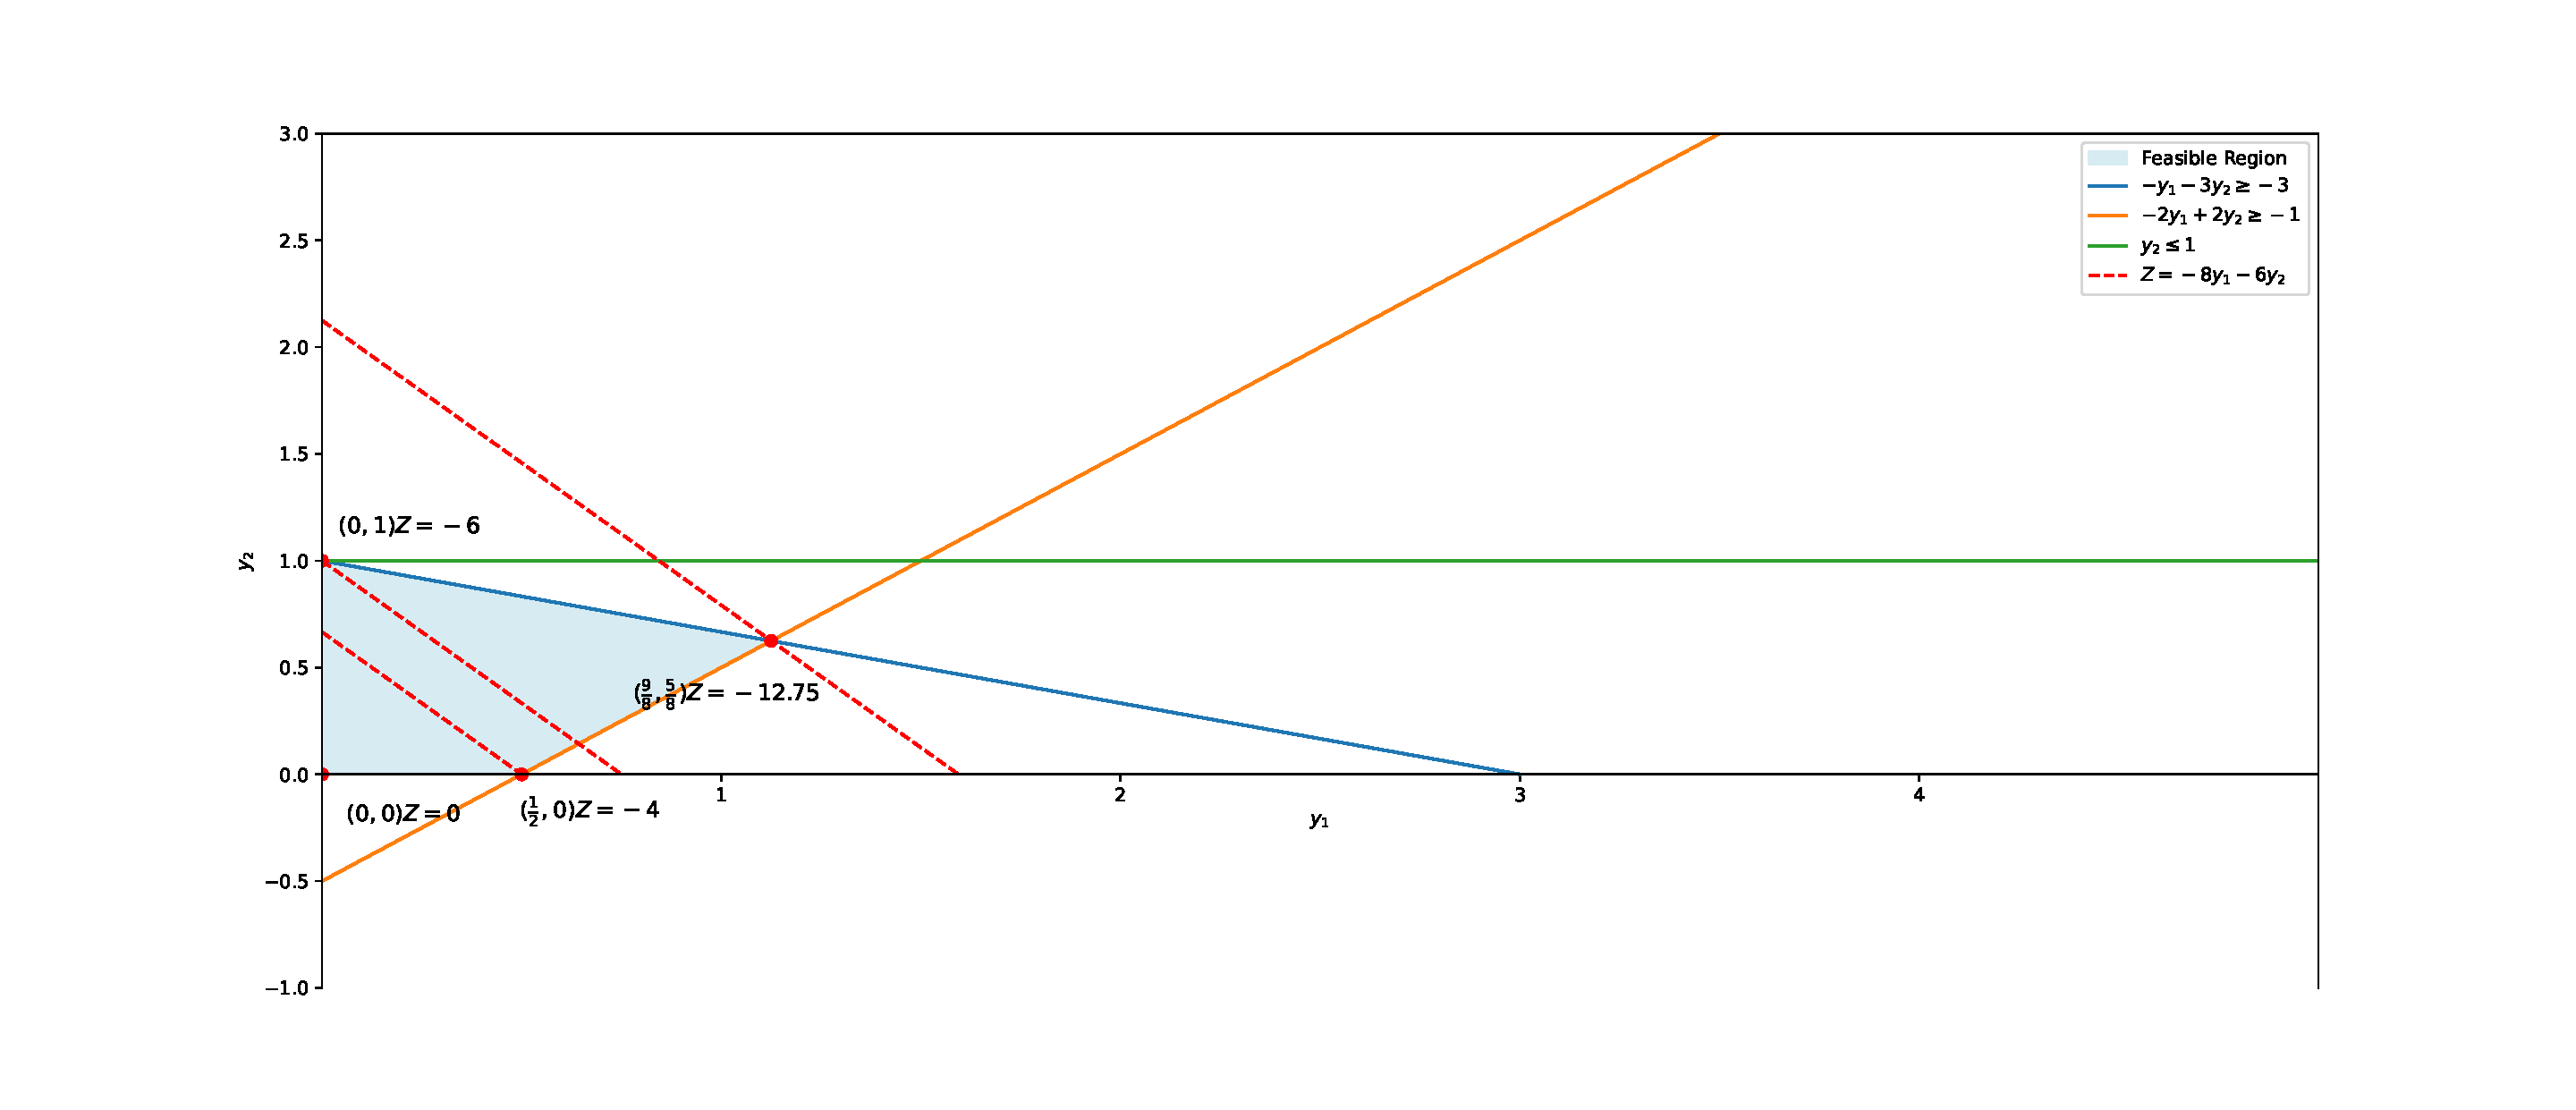
\includegraphics[width=1\textwidth]{Exercices/ex1.1.pdf}
\end{center}

\[\text{solution is} \hspace{0.2cm}\boxed{(x_1,x_2)=(\frac{9}{8},\frac{5}{8})}\]

\begin{minipage}{0.45\textwidth}

\vspace{-1.1cm}
\subsubsection*{\underline{Primal}}
\(X^{*} = \left[\begin{matrix} x^{*}_{1} & x^{*}_{2} & x^{*}_{3}  \end{matrix}\right]\)

\vspace{0.45cm}

\(\text{max } -Z = -3x_1 - x_2 - x_3\)

\vspace{0.45cm}
\(
\left\{
\begin{array}{l}
    -x_{1} - 2x_{2}  \leq -8 \\
    -3x_{1} + 2x_{2} - x_{3} \leq -6 \\
    x_{1}, x_{2}, x_{3}\geq 0
\end{array}
\right.
\)
\end{minipage}
\hfill
\begin{minipage}{0.45\textwidth}

\vspace{-0.3cm}
\subsubsection*{\underline{Dual}}
\(Y^{*} = \left[\begin{matrix} \frac{9}{8} & \frac{5}{8} \end{matrix}\right]\)

\vspace{0.45cm}
\(\text{min } Z = -8y_1 - 6y_2 \)

\vspace{0.45cm}

\(
\left\{
\begin{array}{l}
    -y_{1} - 3y_{2} \geq -3 \\
    -2y_{1} + 2y_{2}  \geq -1 \\
     -y_{2}  \geq -1 \\
    y_{1}, y_{2}\geq 0
\end{array}
\right.
\)
\end{minipage}

\vspace{1.5cm}

\[
\left\{
\begin{array}{l}
    x^{*}_{1}(-(\frac{9}{8}) - 3(\frac{5}{8}) + 3) = 0 \\
    x^{*}_{2} (-2(\frac{9}{8}) + 2(\frac{5}{8})) +1 = 0\\
    x^{*}_3 (-(\frac{5}{8}) + 1) = 0 \\
\end{array}
\right.
\quad
\Longrightarrow
\quad
\left\{
\begin{array}{l}
    x^{*}_{1}(0) = 0 \\
    x^{*}_{2} (0) = 0\\
    x^{*}_3 (\frac{3}{8}) = 0 \\
\end{array}
\right.
\quad
\Longrightarrow
\quad
\left\{
\begin{array}{l}
    x^{*}_{1} > 0 \\
    x^{*}_{2} > 0\\
    x^{*}_3 = 0 \\
\end{array}
\right.
\]

\vspace{0.75cm}

\[
\left\{
\begin{array}{l}
    y^{*}_{1} (-8 -x^{*}_{1}-2x^{*}_{2}) = 0  \\
    y^{*}_{2}(-6 -3 x^{*}_{1}+ 2x^{*}_{2} - x^{*}_{3} ) = 0  \\ 
\end{array}
\right.
\quad
\Longrightarrow
\quad
\left\{
\begin{array}{l}
    \frac{9}{8}(-8 -x^{*}_{1}-2x^{*}_{2}) = 0  \\
    \frac{5}{8}(-6 -3 x^{*}_{1}+ 2x^{*}_{2}) = 0  \\
\end{array}
\right.
\quad
\Longrightarrow
\quad
\left\{
\begin{array}{l}
    -8 -x^{*}_{1}-2x^{*}_{2} = 0  \\
    -6 -3 x^{*}_{1}+2 x^{*}_{2} = 0  \\
\end{array}
\right.

\]

\vspace{0.25cm}

\[
\left\{
\begin{array}{l}
     x^{*}_{1}+2x^{*}_{2} = 8  \\
     3 x^{*}_{1}-2x^{*}_{2} = 6  \\
\end{array}
\right.
\right.
\quad
\Longrightarrow
\quad
\left\{
\begin{array}{l}
    x^{*}_{1} = \frac{7}{2} \\
    x^{*}_{2}= \frac{9}{4} \\
\end{array}
\right.
\]


\vspace{0.75cm}


\[\boxed{X^{*} = \left[\begin{matrix} \frac{7}{2} & \frac{9}{4}  & 0   \end{matrix}\right]}\]

\vspace{1cm}

